\pdfoutput=1
\documentclass{article} % For LaTeX2e
\usepackage{iclr2017_workshop,times}
\usepackage{hyperref}
\usepackage{url}

% my imports
\usepackage{amssymb,amsmath,amsthm}
\usepackage[makeroom]{cancel}
\usepackage{algorithm}
\usepackage[noend]{algpseudocode}
\usepackage{graphicx}
\usepackage{multirow,bigstrut}
\newcommand{\eqname}[1]{\tag*{#1}}

\usepackage{textcomp}

\title{Reinterpreting Importance-Weighted \\Autoencoders}


\author{Chris Cremer, Quaid Morris \& David Duvenaud \\
Department of Computer Science\\
University of Toronto\\
%Toronto, ON, Canada \\
\texttt{\{ccremer,duvenaud\}@cs.toronto.edu} \\
\texttt{\{quaid.morris\}@utoronto.ca}
% \texttt{ccremer@cs.toronto.edu},\texttt{quaid.morris@utoronto.ca},\texttt{duvenaud@cs.toronto.edu}\\
}

\newcommand{\fix}{\marginpar{FIX}}
\newcommand{\new}{\marginpar{NEW}}

\begin{document}


\maketitle

\begin{abstract}
The standard interpretation of importance-weighted autoencoders is that they maximize a tighter lower bound on the marginal likelihood.
We give an alternate interpretation of this procedure: that it optimizes the standard variational lower bound, but using a more complex distribution. 
We formally derive this result, and visualize the implicit importance-weighted approximate posterior.
%This distribution, $q_{IW}(z|x)$, is an importance weighted distribution implicitly defined by the  a pointwise reweighting of a parametric base distribution $q(z|x)$.
%We also propose a family of extensions allowing iterative refinement of the approximate posterior based on gradients of the log-likelihood.
\end{abstract}
 

\begin{figure}[b]
  \centering
  \quad True posterior \quad  \qquad $q_{IW}$ with $k=1$  \quad \qquad $q_{IW}$ with $k=10$  \qquad $q_{IW}$ with $k=100$
      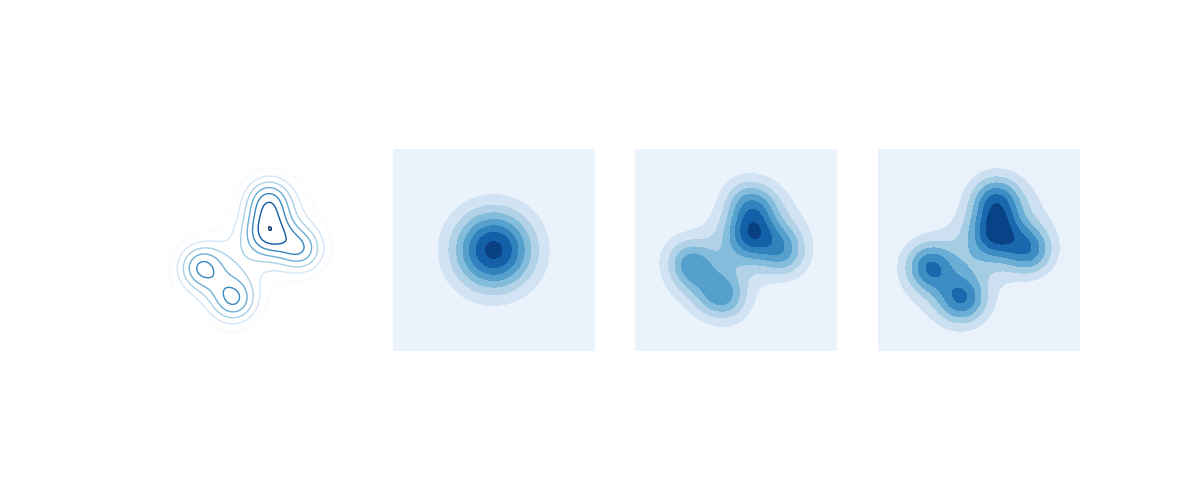
\includegraphics[width=1.\textwidth, clip, trim=2.5cm 3.9cm 2cm 3.6cm]{figs/figure_1.png}
  \vspace{-5mm}
  \caption{Approximations to a complex true distribution, defined via sampling-importance-resampling. As $k$ grows, this approximation approaches the true distribution.}
  \label{viz1}
\end{figure}


\section{Background}
The importance-weighted autoencoder (IWAE; \cite{burda2015importance}) maximizes the following multi-sample evidence lower bound (ELBO): 
\begin{align} 
    log(p(x)) &
    % log\left(E_{z_{1}...z_{k} \sim q(z|x)} \left[  \frac{1}{k}\sum_{i=1}^k \frac{p(x,z_i)}{q(z_i|x)}    \right]   \right)_{ML}
    % \\
    % & 
    \geq E_{z_{1}...z_{k} \sim q(z|x)} \left[log\left(  \frac{1}{k}  \sum_{i=1}^k \frac{p(x,z_i)}{q(z_i|x)}  \right)  \right] = L_{IWAE}[q] \label{iwae_elbo}  \eqname{(IWAE ELBO)}
\end{align}
which is a tighter lower bound than the ELBO maximized by the variational autoencoder (VAE; \cite{vae}):
\begin{align}
    log(p(x)) & \geq E_{z_{1}...z_{k} \sim q(z|x)} \left[  \frac{1}{k}\sum_{i=1}^k log\left(\frac{p(x,z_i)}{q(z_i|x)}  \right)  \right] = L_{VAE}[q]. \label{vae_elbo} \eqname{(VAE ELBO)}
\end{align}
Here we've written the VAE bound as a multisample lower bound to compare it to the IWAE bound. The following equations are the gradients of the VAE ELBO and the IWAE ELBO, respectively:
\begin{align} 
    \nabla_{\Theta} \mathcal{L}_{VAE}[q] &= E_{z_{1}...z_{k} \sim q(z|x)} \left[   \sum_{i=1}^k \frac{1}{k} \nabla_{\Theta} log\left(\frac{p(x,z_i)}{q(z_i|x)}  \right)  \right] \label{vae_grad} \\
% \end{align}
% \begin{align} 
    \nabla_{\Theta} \mathcal{L}_{IWAE}[q] &= E_{z_{1}...z_{k} \sim q(z|x)} \left[  \sum_{i=1}^k \tilde{w}_i \nabla_{\Theta} log\left(\frac{p(x,z_i)}{q(z_i|x)}  \right)  \right] \label{iwae_grad}
\end{align}
where $$\tilde{w}_i = \frac{\frac{p(x,z_i)}{q(z_i|x)}}{\sum_{j=1}^k \frac{p(x,z_j)}{q(z_j|x)}}.$$
From equations \eqref{vae_grad} and \eqref{iwae_grad}, we see that the gradient of the VAE ELBO evenly weights the samples, whereas the IWAE gradient weights the samples based on their relative importance $\tilde{w}_i$.




% \section{Defining the implicit distribution q\textsubscript{IW}}

\section{Defining the implicit distribution \texorpdfstring{$q_{IW}$}{}}

%From the gradient of the IWAE bound (Eqn. \ref{iwae_grad}), we know that each sample is weighted by their importance $\tilde{w}_i$. This weighting implicitly defines a nonparametric approximate posterior.

In this section, we derive the implicit distribution that arises from importance sampling from a distribution $p$ using $q$ as a proposal distribution.

Given a batch of samples $z_{1}...z_{k}$ from $q(z|x)$, the following is the importance weighted $q_{IW}$ distribution as a function of one of the samples, $z_i$:
\begin{align} 
    q_{IW}(z_i|x,z_{\setminus i}) &= k \tilde{w}_i q(z_i|x)
    = \left( \frac{ \frac{p(x,z_i)}{q(z_i|x)}}{  \frac{1}{k}   \sum_{j=1}^k \frac{p(x,z_j)}{q(z_j|x)}}  \right) q(z_i|x) 
    = \frac{p(x,z_i)}{\frac{1}{k}   \sum_{j=1}^k \frac{p(x,z_j)}{q(z_j|x)}} 
\end{align}
The marginal distribution $q_{IW}(z|x)$ is given by:
\begin{align} 
    % q_{IW}(z|x) &= E_{z_{1}...z_{k} \sim q(z|x)} \left[ q_{IW}(z|x, z_{\setminus i}) \right] \textnormal{for any $i$}. \\
    q_{IW}(z|x) &= E_{z_{2}...z_{k} \sim q(\cdot |x)} \left[ \frac{p(x,z)}{  \frac{1}{k} \left( \frac{p(x,z)}{q(z|x)}+ \sum_{j=2}^k \frac{p(x,z_j)}{q(z_j|x)} \right) } \right] \label{marg} %\textnormal {where $z_1 = z$}. 
\end{align}





% \begin{align} 
%     q_{IW}(z_i|x,z_{\setminus i}) &= k \tilde{w}_i q(z_i|x)
%     = \left( \frac{ \frac{p(x,z_i)}{q(z_i|x)}}{\frac{1}{k}   \sum_{j=1}^k \frac{p(x,z_j)}{q(z_j|x)} } \right) q(z_i|x) 
%     = \frac{p(x,z_i)}{\frac{1}{k}   \sum_{j=1}^k \frac{p(x,z_j)}{q(z_j|x)}} 
% \end{align}
% The marginal distribution $q_{IW}(z|x)$ is given by:
% \begin{align} 
%     % q_{IW}(z|x) &= E_{z_{1}...z_{k} \sim q(z|x)} \left[ q_{IW}(z|x, z_{\setminus i}) \right] \textnormal{for any $i$}. \\
%     q_{IW}(z|x) &= E_{z_{1}...z_{k} \sim q(z|x)} \left[ \frac{p(x,z)}{\frac{1}{k}   \sum_{j=1}^k \frac{p(x,z_j)}{q(z_j|x)}} \right] \textnormal{where $z_1 = z$}. 
% \end{align}


 
When $k=1$, $q_{IW}(z|x)$ will be equal to $q(z|x)$.
When $k > 1$, we see that the form of $q_{IW}$ depends on the true posterior $p$. 
When $k=\infty$, $q_{IW}(z|x)$ becomes the true posterior $p(z|x)$.
See the Appendix for details.
Note that, to evaluate $q_{IW}$, we require an integral over batches of samples $z_{2}...z_{k}$ from $q(z|x)$. Since this integral is intractable, $q_{IW}$ must be approximated by a finite number of batches.

Figure \ref{viz1} visualizes $q_{IW}$ on a 2D distribution approximation problem. The base distribution $q$ is a Gaussian.  As we increase the number of samples $k$ used for the sampling-resampling, the approximation approaches the true distribution. This distribution is nonparametric in the sense that, as the true posterior grows more complex, so does the shape of $q_{IW}$.

%The marginal distribution $q_{IW}(z|x)$ is the same distribution that we would sample from if 

\subsection{Recovering the IWAE bound from the VAE bound}

Here we show that the IWAE ELBO is equivalent to the VAE ELBO, but with a more flexible $q_{IW}$ distribution, implicitly defined by importance reweighting.
First, we start by writing the VAE ELBO in its minibatch form, as an average over $k$ samples:
\begin{align} 
    \log p(x) &\geq 
    \mathcal{L}_{VAE}[q] &=
    E_{z \sim q(z|x)} \left[  log\left(\frac{p(x,z)}{q(z|x)} \right) \right]  
    &= E_{z_{1}...z_{k} \sim q(z|x)} \left[  \frac{1}{k}\sum_{i=1}^k log\left(\frac{p(x,z_i)}{q(z|x)} \right) \right]
\end{align}
If we now set $q(z|x) = q_{IW}(z|x)$, then we recover the IWAE ELBO:
\begin{align}
        \mathcal{L}_{VAE}[q_{IW}]
        &= E_{z_{1}...z_{k} \sim q_{IW}(z|x)} \left[  \frac{1}{k}\sum_{i=1}^k log\left(\frac{p(x,z_i)}{q_{IW}(z_i|x,z_{\setminus i})}  \right)  \right] \\
    &= E_{z_{1}...z_{k} \sim q(z|x)} \left[ \sum_{l=1}^k \tilde w_l \frac{1}{k}\sum_{i=1}^k log\left(\frac{p(x,z_i)}{\frac{p(x,z_i)}{\frac{1}{k}   \sum_{j=1}^k \frac{p(x,z_j)}{q(z_j|x)}}}  \right)  \right] \\
    %&= E_{z_{1}...z_{k} \sim (z|x)} \left[ \frac{1}{k}\sum_{i=1}^k log\left(\frac{1}{k} \sum_{j=1}^k \frac{p(x,z_j)}{q(z_j|x)}\right)  \right] \label{with_avg} \\   
    &= E_{z_{1}...z_{k} \sim q(z|x)} \left[  log\left(\frac{1}{k}\sum_{j=1}^k \frac{p(x,z_j)}{q(z_j|x)}  \right)  \right] = \mathcal{L}_{IWAE}[q]
\end{align}
%Eqn. \ref{without_avg} follows Eqn. \ref{with_avg} since nothing is indexed by $i$ within the outer sum over indexes $i$.
Thus we see that VAE with $q_{IW}$ is equivalent to the IWAE ELBO.  For a more detailed derivation, see the Appendix.

%The implicit variational distribution of the IWAE ELBO is a stochasticaly weighted version of the variational distribution $q(z|x)$, where the optimal weighting is $p(z|x) / q(z|x)$. 





% \section{Sampling q\textsubscript{IW}}
\section{Sampling \texorpdfstring{$q_{IW}$}{}}



%Due to the importance weighting of the lower bound, we can no longer sample from the orginal variational distribution $q(z|x)$; we must sample $q_{IW}$. 
The procedure to sample from $q_{IW}(z|x)$ is shown in Algorithm \ref{algo1}.
It is equivalent to sampling-importance-resampling (SIR). 
%What does $q_{IW}(z|x)$ look like? 



\begin{figure*}[t]
\centering
\begin{centering}
\begin{minipage}[t]{0.49\columnwidth}
\begin{algorithm}[H]
\caption{Sampling from $q_{IW}$}\label{algo1}
\begin{algorithmic}[1]
    \State $\textit{k} \gets \textit{number of samples}$
    \State $q(z|x) = f_\phi(x)$
    \For {$i$ in $1 \dots k$}
        \State $z_i \sim q(z|x)$
        \State $w_i = \frac{p(x,z_i)}{q(z_i|x)}$
    \EndFor    
    \State Each $\tilde w = w_i/\sum_{i=1}^{k} w_i$
    \State $j \sim Cat(\tilde{w})$
    \State Return $z_j$
\end{algorithmic}
\end{algorithm}
\end{minipage}
\end{centering}

%\hfill
%\begin{minipage}[t]{0.49\columnwidth}
%\begin{algorithm}[H]
%\caption{Sampling from recurrent $q_{IW}$}\label{algo2}
%\begin{algorithmic}[1]
%    \State $\textit{k} \gets \textit{number of samples}$
%    \For {$i$ in $1 \dots k$}
%        \State $q_i(z|x) = f_\phi(x, \nabla_z logp(z_{i-1}, x_{i-1}))$
%        \State $z_i \sim q_i(z|x)$
%        \State $w_i = \frac{p(x,z_i)}{q(z_i|x)}$
%    \EndFor    
%    \State Each $\tilde w = w_i/\sum_{i=1}^{k} w_i$
%    \State $j \sim Cat(\tilde{w})$
%    \State Return $z_j$
%\end{algorithmic}
%\end{algorithm}
%\end{minipage}
\hfill
\caption{Algorithm 1 defines the procedure to sample from $q_{IW}$.
%Algorithm 2 is a proposed extension using a recurrent model.
}
\end{figure*}





\section{Resampling for prediction}
%Sampling from the recognition distribution $q$ of the IWAE model can be split into two parts: sampling for training, and sampling for evaluation. 
During training, we sample the $q$ distribution and implicitly weight them with the IWAE ELBO. After training, we need to explicitly reweight samples from $q$.

\begin{figure}[h]
  \centering
      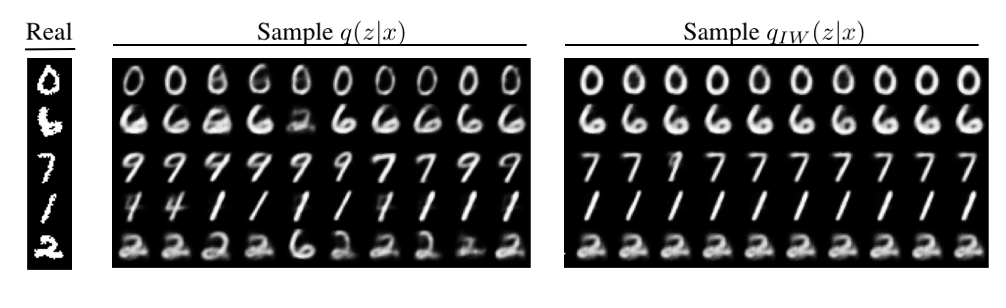
\includegraphics[width=1.\textwidth, clip, trim=0cm .5cm 0cm 0cm]{figs/samps.png}
  \caption{Reconstructions of MNIST samples from $q(z|x)$ and $q_{IW}$. The model was trained by maximizing the IWAE ELBO with K=50 and 2 latent dimensions. The reconstructions from $q(z|x)$ are greatly improved with the sampling-resampling step of $q_{IW}$.}
  \label{recon}
\end{figure}

In Fig. \ref{recon}, we demonstrate the need to sample from $q_{IW}$ rather than $q(z|x)$ for reconstructing MNIST digits. We trained the model to maximize the IWAE ELBO with K=50 and 2 latent dimensions, similar to Appendix C in \cite{burda2015importance}. When we sample from $q(z|x)$ and reconstruct the samples, we see a number of anomalies. However, if we perform the sampling-resampling step (Algo. \ref{algo1}), then the reconstructions are much more accurate. The intuition here is that we trained the model with $q_{IW}$ with $K=50$ then sampled from $q(z|x)$ ($q_{IW}$ with $K=1$), which are very different distributions, as seen in Fig. \ref{viz1}.



\section{Discussion}

\cite{bachman} also showed that the IWAE objective is equivalent to stochastic variational inference with a proposal distribution corrected towards the true posterior via normalized importance sampling. In other words, the IWAE lower bound can be interpreted as the standard VAE lower bound with an implicit $q_{IW}$ distribution. We build on this idea by further examining $q_{IW}$ and by providing visualizations to help better grasp the interpretation. In light of this, IWAE can be seen as increasing the complexity of the approximate distribution $q$, similar to other methods that increase the complexity of $q$, such as Normalizing Flows (\cite{normflow}), Variational Boosting (\cite{varboosting}) or Hamiltonian variational inference (\cite{salimans2015markov}). With this interpretation in mind, we can generalize $q_{IW}$ to be more broadly applicable to any divergence measure. An interesting avenue of future work is the comparison of IW-based variational families with alpha-divergences or operator variational objectives. 

% They showed this by using a “meta” auxiliary distribution formed by applying a normalized importance sampling correction to q. 

% We extend their work by further developping / more directly relating the interpretation of the IWAR and VAE bounds. 

% with more vizualizations, emphazizing the need to sample q_IW. 

% We showed that the IWAE lower bound can be interpreted as the standard VAE lower bound with an implicit $q_{IW}$ distribution.



% We retell a similar story through a differnt light.

%, and Real NVP (\cite{realnvp}).

 

%We show that the IWAE framework can be extended to have richer families of base distributions, which can be jointly dependent or even based on recurrent neural networks. See \cite{local}











% \newpage

% \section{Other}


% \begin{itemize}
%     \item We show that the IWAE lower bound can be interpreted as the standard VAE lower bound with a nonparametric, implicit $q$ distribution.
%     \item We show that the sampling-resampling step, which samples from this implicit distribution, is necessary to produce samples from the variational posterior.  
    
%     % This step resolves an anomaly in the original IWAE paper.
%     \item We show that the IWAE framework can be extended to have richer families of base distributions, which can be jointly dependent or even based on recurrent neural networks.
% \end{itemize}

% % We notice that this point appears be overlooked in other works as well. \cite{maddison2016concrete}

% We provided a different interpretation of IWAE: its the same elbo, but different q. 









 
% something about the rnn  \\
% This is important because .. \\
% fig one will be IWSI \\
% The only difference between the variational autoencoder (VAE; \cite{vae}) and the importance weighted autoencoder (IWAE; \cite{burda2015importance}) is their evidence lower bounds (ELBOs). Although the variational distribution $q_\phi(z|x)$ is typically a Normal distribution, the multi-sample IWAE ELBO implicitly defines a variational distribution that differs from a Normal distribution. (Something about people sample q not q iwae)\\ 
% Here we reinterpret the \\ 
% Here, we define the formula of the distribution, how to sample from it, visualize intermediate distributions, and samples from the distribution.\\
% The following are the multi-sample equations for the log evidence (marginal likelihood), IWAE ELBO, and VAE ELBO, respectively. 

%However, this interpretation is incomplete if we do not also consider that the implicit $q$ distribution is more complex.

% This is an analysis of the implicit variational distribution defined by the IWAE ELBO \citep{burda2015importance}. I define the formula of the distribution, how to sample from it, and visualize intermediate distributions, and samples from the distribution...

% \newpage














\subsubsection*{Acknowledgments}

We'd like to thank an anonymous ICLR reviewer for providing insightful future directions for this work.

\bibliography{iclr2017_workshop}
\bibliographystyle{iclr2017_workshop}


\section{Appendix}




\subsection{Detailed derivation of equivalence of VAE and IWAE bound.}
\label{detailed_derivation}

First, we start by writing the VAE ELBO in its minibatch form, as an average over $k$ samples:
\begin{align} 
    \log p(x) &\geq 
    \mathcal{L}_{VAE}[q] =
    E_{z \sim q(z|x)} \left[  log\left(\frac{p(x,z)}{q(z|x)} \right) \right]  
    &= E_{z_{1}...z_{k} \sim q(z|x)} \left[  \frac{1}{k}\sum_{i=1}^k log\left(\frac{p(x,z_i)}{q(z|x)} \right) \right]
\end{align}
If we now set $q(z|x) = q_{IW}(z|x)$, then we recover the IWAE ELBO:
\begin{align}
    L_{VAE}[q_{IW}] &= E_{z_{1}...z_{k} \sim q_{IW}(z|x)} \left[  \frac{1}{k}\sum_{i=1}^k log\left(\frac{p(x,z_i)}{q_{IW}(z_i|x,z_{\setminus i})}  \right)  \right] \\
    &= E_{z_{1}...z_{k} \sim q_{IW}(z|x)} \left[  \frac{1}{k}\sum_{i=1}^k log\left(\frac{p(x,z_i)}{\frac{p(x,z_i)}{\frac{1}{k}   \sum_{j=1}^k \frac{p(x,z_j)}{q(z_j|x)}}}  \right)  \right] \\
    &= E_{z_{1}...z_{k} \sim q_{IW}(z|x)} \left[  \frac{1}{k}\sum_{i=1}^k log\left(\frac{1}{k} \sum_{j=1}^k \frac{p(x,z_j)}{q(z_j|x)}\right)  \right] \label{with_i} \\
    &= E_{z_{1}...z_{k} \sim q_{IW}(z|x)} \left[ log\left(\frac{1}{k} \sum_{j=1}^k \frac{p(x,z_j)}{q(z_j|x)}\right)  \right]  \label{without_i} \\
    &= E_{z_{1}...z_{k} \sim q(z|x)} \left[  \sum_{l=1}^k \tilde w_l  \left( log\left(\frac{1}{k} \sum_{j=1}^k \frac{p(x,z_j)}{q(z_j|x)}\right)\right)  \right] \label{with_w} \\ 
    &= E_{z_{1}...z_{k} \sim q(z|x)} \left[  log\left(\frac{1}{k}\sum_{j=1}^k \frac{p(x,z_j)}{q(z_j|x)}  \right)  \right] = \mathcal{L}_{IWAE}[q] \label{without_w}
\end{align}
Eqn. \ref{without_i} follows Eqn. \ref{with_i} since index $i$ is not present within the sum over $i$. Similarly, from Eqn. \ref{with_w} to Eqn. \ref{without_w}, index $l$ is not present within the sum over $l$ and $\sum_{l=1}^k \tilde w_l$ sums to one. Eqn. \ref{without_w} is the IWAE ELBO, thus we see that VAE with $q_{IW}$ is equivalent to the IWAE ELBO.















\subsection{Proof that \texorpdfstring{$q_{IW}$}{} is closer to the true posterior than \texorpdfstring{$q$}{}}

Section \ref{detailed_derivation} showed that $\mathcal{L}_{IWAE}(q) = \mathcal{L}_{VAE}(q_{IW})$. That is, the IWAE ELBO with the base $q$ is equivalent to the VAE ELBO with the importance weighted $q_{IW}$. Due to Jensen\textquotesingle s Inequality and as shown in \cite{burda2015importance}, we know that the IWAE ELBO is an upper bound of the VAE ELBO: ${L}_{IWAE}(q) \geq {L}_{VAE}(q)$. Furthermore, the log marginal likelihood can be factorized into: $log(p(x)) = {L}_{VAE}(q) + KL(q||p)$, and rearranged to: $KL(q||p) = log(p(x)) - {L}_{VAE}(q)$.

Following the observations above and substituting $q_{IW}$ for $q$:
\begin{align} 
    KL(q_{IW}||p) &= log(p(x)) - {L}_{VAE}(q_{IW}) \\
    &= log(p(x)) - {L}_{IWAE}(q) \\
    &\leq log(p(x)) - {L}_{VAE}(q) = KL(q||p)
\end{align}
Thus, $KL(q_{IW}||p) \leq KL(q||p)$, meaning $q_{IW}$ is closer to the true posterior than $q$ in terms of KL divergence. 

Another perspective is in the limit of ${k=\infty}$. Recall that the marginal likelihood can be approximated by importance sampling:
\begin{align} 
    p(x) &= E_{q(z|x)}\left[\frac{p(x,z)}{q(z|x)} \right] \approx \frac{1}{k}\sum_i^k \frac{p(x,z_i)}{q(z_i|x)}
\end{align}
where $z_i$ is sampled from $q(z_i|x)$. Thus, the denominator of Eqn. \ref{marg} is approximating $p(x)$. As $k$ approaches infinity, $q_{IW}$ approaches the true posterior $p(z|x)$.



% Thus, when $k=\infty$:
% \begin{align} 
%     q_{IW}(z|x) &= 
%     E_{z_{1}...z_{\infty} \sim q(z|x)} \left[ \frac{p(x,z)}{\lim_{k\to\infty} \frac{1}{k} \sum_{j=1}^k \frac{p(x,z_j)}{q(z_j|x)}} \right] %\textnormal {where $z_1 = z$}
%     = \frac{p(x,z)}{E_{q(z|x)}\left[\frac{p(x,z)}{q(z|x)} \right]}
%     = \frac{p(x,z)}{p(x)} 
%     = p(z|x)
% \end{align}
% Thus $q_{IW}(z)$ is equal to the true posterior $p(z|x)$ when $k=\infty$, as expected.


Another way to write it:
\begin{align}
q_{IW}(z_i|x,z_{\setminus i}) =  \frac{p(x)}{  \frac{1}{k} \left( \frac{p(x,z_i)}{q(z_i|x)}+ \sum_{j=2}^k \frac{p(x,z_j)}{q(z_j|x)} \right) }  p(z_i|x)
\end{align}

\begin{align} 
    % q_{IW}(z|x) &= E_{z_{1}...z_{k} \sim q(z|x)} \left[ q_{IW}(z|x, z_{\setminus i}) \right] \textnormal{for any $i$}. \\
    q_{IW}(z|x) &= E_{z_{2}...z_{k} \sim q(\cdot |x)} \left[ \frac{p(x)}{  \frac{1}{k} \left( \frac{p(x,z)}{q(z|x)}+ \sum_{j=2}^k \frac{p(x,z_j)}{q(z_j|x)} \right) } \right] p(z|x) \label{marg1} %\textnormal {where $z_1 = z$}. 
\end{align}




\section{Visualizing \texorpdfstring{$q_{IW}$}{} in 1D}

We can look at the intermediate variational distributions with different numbers of samples $k$ in 1 dimension.
Figure~\ref{viz2} demonstrates how the approximate posterior approaches the true posterior as $k$ increases. 

\begin{figure}[H]
  \centering
      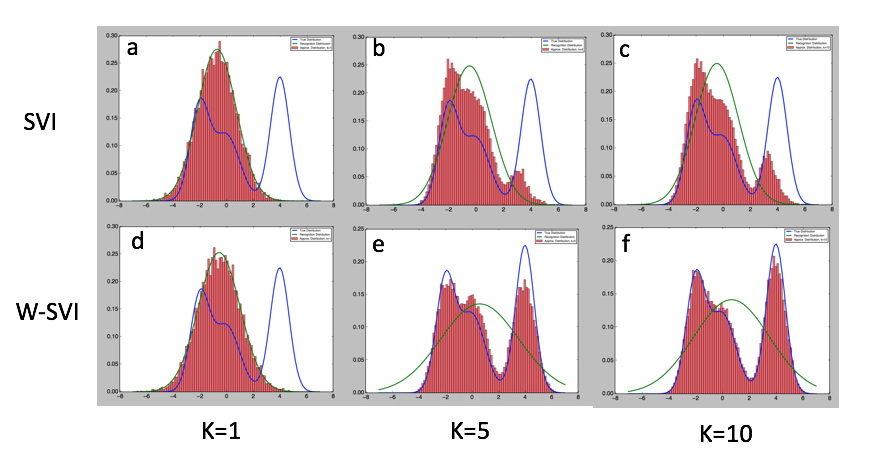
\includegraphics[width=1.\textwidth]{figs/posteriors.png}
  \caption{Visualization of the importance weighted posterior. The blue distribution is the intractable distribution that we are trying to approximate. The green distribution is the variational distribution. The variational distributions of a, b, and c were optimized via SVI, whereas d, e, and f were optimized with SVI with the IWAE ELBO. The red histograms are importance weighted samples from the variational distribution.}
  \label{viz2}
\end{figure}




% \begin{figure}[H]
% \centering
%     \begin{tabular}{ccccccccccccccccccccccccccccccc}
        
%         % 1&2&3&4&5&6&7&8&9&10&11&12&13&14&15&16&17&18&19&20\\
%         &Real&&&&&&Sample $q(z|x)$&&&&&&&&&Sample $q_{IW}(z|x)$&&&&&&&&&&&\\        
%         % \cline{2-2} \cline{4-12} \cline{14-21}
        
%         \multicolumn{30}{c}{\includegraphics[scale=.7]{figs/recon_iwae.png}}\\
        
%         % a&c&c&d&c&d

%     \end{tabular}
% \caption{Visualization of the reconstructions of samples from }
% \label{recon}
% \end{figure}





\end{document}











% \begin{figure}[H]
% % \begin{table}[ht]

% \centering
% % \renewcommand{\arraystretch}{3}
%     \begin{tabular}{cccc}
        
%         % & \multicolumn{1}{c}{VAE} & & \multicolumn{4}{c}{IWAE} \\
        
%         & Sample $q(z|x)$ & & Sample $q_{IWAE}$ \\
%         \cline{2-2}  \cline{4-4} \\
%         % \rule{0pt}{3ex}
        
%         % 1 & 2 & 3 & 4 \\
        
%         % \rotatebox{90}{VAE\ }\vline  & \multirow{2}{*}{\includegraphics[width=45mm]{figs/recon_samplingvae.png}} & & \multirow{2}{*}{\includegraphics[width=45mm]{figs/recon_samplingiwae.png}} \\[4.5ex]
        
%         % \rotatebox{90}{IWAE\ }\vline & & & \\[4.5ex]        
        
%         % \cline{1-1}
    
%         VAE\ \ \ \ \vline  & \multirow{2}{*}{\includegraphics[width=45mm]{figs/recon_samplingvae.png}} & & \multirow{2}{*}{\includegraphics[width=45mm]{figs/recon_samplingiwae.png}} \\[9.5ex]
        
%         \\
        
%         IWAE\ \vline & & & \\[9ex]
        
%         \\
%     \end{tabular}
% \caption{Visualization of the reconstructions of samples from $q(z|x)$ (left) and $qIWAE$ (right). K indicates the number of samples and VAE/IWAE indicates the ELBO used during training. 2latent dimensions, k=50}
% % \label{tab:gt}
% % \end{table}
% \label{recon}
% \end{figure}



% q in elbo

% \begin{align} 
%     log(p(x)) & \geq E_{z_{1}...z_{k} \sim q(z|x)} \left[  \frac{1}{k}\sum_{i=1}^k log\left(\frac{p(x,z_i)}{q_{IWAE}(z_i|x)}  \right)  \right] \\
%     &= E_{z_{1}...z_{k} \sim q(z|x)} \left[  \frac{1}{k}\sum_{i=1}^k log\left(\frac{p(x,z_i)}{E_{z_{1}...z_{k} \sim q(z|x)} \left[\frac{p(x,z_i)}{\frac{1}{k}\sum_i^k \frac{p(x,z_j)}{q(z_j|x)}}  \right]}  \right)  \right] \label{with_e} \\
%     &= E_{z_{1}...z_{k} \sim q(z|x)} \left[  \frac{1}{k}\sum_{i=1}^k log\left(\frac{p(x,z_i)}{\left(\frac{p(x,z_i)}{\frac{1}{k}\sum_j^k \frac{p(x,z_j)}{q(z_j|x)}}  \right)}  \right)  \right] \label{without_e} \\
%     &= E_{z_{1}...z_{k} \sim q(z|x)} \left[  \frac{1}{k}\sum_{i=1}^k log\left(\frac{1}{k}\sum_{j=1}^k \frac{p(x,z_j)}{q(z_j|x)}  \right)  \right] \label{with_avg} \\
%     &= E_{z_{1}...z_{k} \sim q(z|x)} \left[  log\left(\frac{1}{k}\sum_{j=1}^k \frac{p(x,z_j)}{q(z_j|x)}  \right)  \right] \label{without_avg}
% \end{align}


% The  standard  interpretation  of  importance-weighted  autoencoders  is  that  they maximize a tighter lower bound on the marginal likelihood.  We give an alternate interpretation: that it optimizes the standard variational lower bound, but using a more complex distribution. This distribution is a stochastic pointwise reweighting of the base variational distribution.  We formally derive this result, and examine properties of the implicit importance weighted posterior.  We also stress the needto use a resampling step to sample from the approximate posterior trained usingthe IWAE objective